\section{Ergebnisse der Betriebsszenarien}
In diesem Teil werden die Auswertung der aufgestellten im Kapitel \ref{s:Betriebsszenarien} ausgewertet und miteinander verglichen.

Obwohl der Unterschied zwischen Betriebskosten gleichmäßig ist, hat unter allen Betriebsszenarien das zweite die höchsten Gesamtbetriebskosten.
60 \% der Kosten entstehen durch wasserstoffbetriebene-Flugzeuge. Drittes Szenario hat der niedrigste Betriebswert von allen drei.

Nennenswert ist das in der Berechnung von allen Betriebsszenarien sind erstmal nur einmalige Infrastrukturausgaben 
ohne jährliche Abschreibungen ausgerechnet. In der Tabelle \ref{Infrastrukturwerte_res} sind die benötigten Werte für jedes Szenario dargestellt.

\begin{table}[h]
	\begin{center}
    \caption{Infrastrukturwerte für alle Szenarien}
	\label{Infrastrukturwerte_res}
	\begin{tabular}{|l|c|c|c|}
		\hline
		 & \textbf{Szenario I}& \textbf{Szenario II}& \textbf{Szenario III} \\ \hline
		Anzahl Ladestationen $n_{BSS}$ & 20 & 10& 14\\ \hline
		Anzahl Batterien $n_{Bat}$ & 101 & 51& 70 \\ \hline
		Anzahl Betankungswagen $n_{BW}$ & 4 & 7 & 5\\ \hline
		Anzahl Pumpen $n_{kP}$  & 5 & 8 & 6\\ \hline
	\end{tabular}
    \end{center}
\end{table}

Das erste Szenario hat die kleinsten Ausgaben, wobei das Szenario Nummer zwei die größte. Szenario zwei ist 27 \% höher als das erste.
Die Gesamtkosten für das zweite Szenario liegen über 35 Tausend Euro.
\begin{figure}[h]
	\centering
	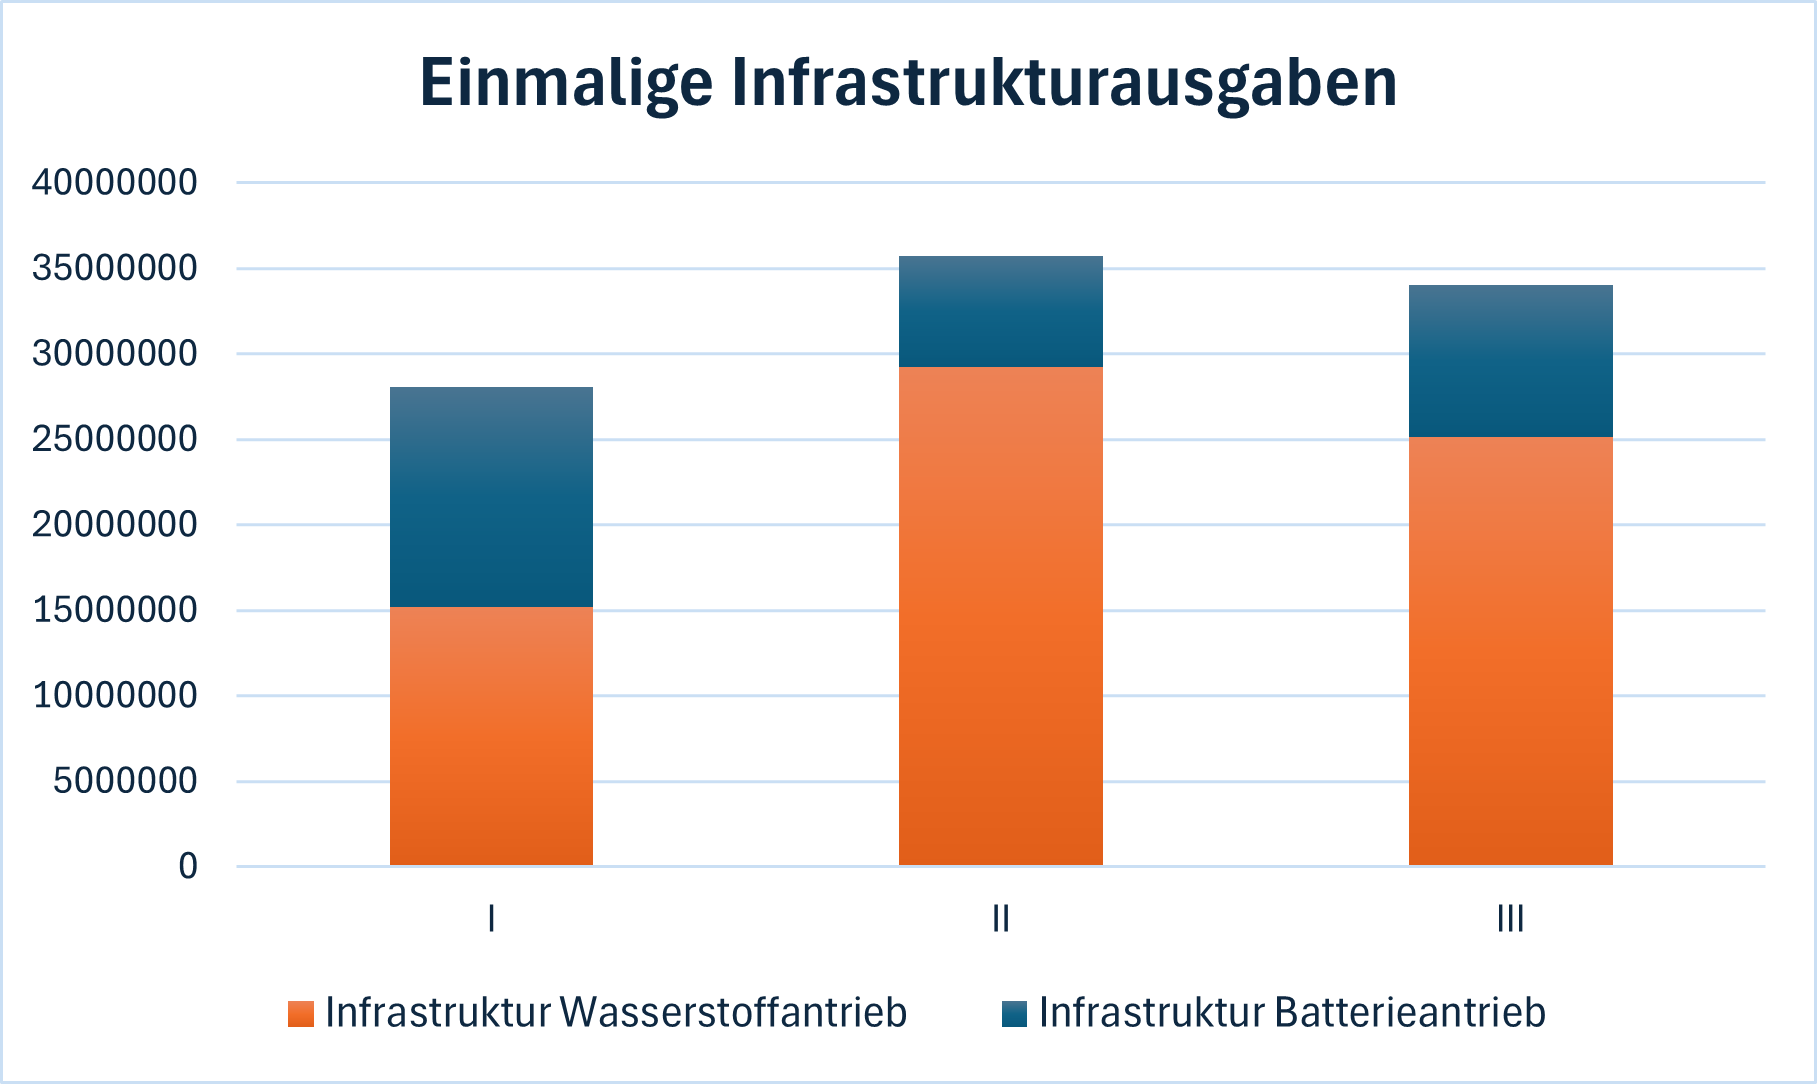
\includegraphics[width=0.8\linewidth]{Bilder/Infr_Szenarien.png}
	\caption[Betriebsszenarien]{Vergleich der einmaligen Infrastrukturausgaben zwischen den Betriebsszenarien}
	\label{res_betriebsszenarien}
\end{figure}